\chapter{Implementacija i korisničko sučelje}
		
		
		\section{Korištene tehnologije i alati}
		
			%\textbf{\textit{dio 2. revizije}}
			
			 %\textit{Detaljno navesti sve tehnologije i alate koji su primijenjeni pri izradi dokumentacije i aplikacije. Ukratko ih opisati, te navesti njihovo značenje i mjesto primjene. Za svaki navedeni alat i tehnologiju je potrebno \textbf{navesti internet poveznicu} gdje se mogu preuzeti ili više saznati o njima}.
			 
			 \normalsize{Komunikacija među članovima tima najvećim je dijelom ostvarena putem platforme  \underline{Discord},\footnote{https://discord.com/} dok su pojedini kraći sastanci nakon konzultacija/demonstracija održani na platformi \underline{MS Teams}.\footnote{https://www.microsoft.com/hr-hr/microsoft-365/microsoft-teams/group-chat-software/}
			 	
			 Za dizajn izgleda aplikacije korišten je software \underline{Adobe XD},\footnote{https://www.adobe.com/products/xd.html}
			 a za izradu UML dijagrama \underline{Astah}.\footnote{https://astah.net/}
			 \underline{Git}\footnote{https://git-scm.com/} je služio kao sustav za upravljanje izvornim kodom na projektu čiji je udaljeni repozitorij smješten na web platformi \underline{GitLab}.\footnote{https://about.gitlab.com/}
			 \newline Uređivanje dokumentacije odvijalo se u okruženju \underline{TeXstudio},\footnote{https://www.texstudio.org/} a jedan od uređivača za pisanje programa za samu aplikaciju bio je \underline{Visual Studio Code}.\footnote{https://code.visualstudio.com/}
			 
			 Za razvoj \textit{frontenda} korišteni su \underline{Dart}\footnote{https://dart.dev/} i \underline{Flutter}.\footnote{https://flutter.dev/} 
			 Dart je programski jezik optimiziran za izgradnju UI-a s posebnim dodatcima kao što su \textit{spread operator} i \textit{collection if} koji omogućavaju lakšu prilagodbu UI-a nekoj platformi, pritom imajući poznatu sintaksu koju je lako svladati. Flutter je Google-ov UI alat za programiranje u Dartu koji se hvali mogućnošću brzog razvoja iznimno vizualno privlačnih aplikacija koje mogu biti mobilne, web ili desktop.
			 
			 Za razvoj \textit{backenda} korišten je \underline{Java Spring \textit{framework}}\footnote{https://spring.io/} (radni okvir). Spring je brz, fleksibilan i siguran okvir za rad s DAO, a poznat je po MVC obrascu korištenjem anotacija.
			 
			 Baza podataka je relacijska baza podataka napravljena putem \underline{PostgreSQL}\footnote{https://www.postgresql.org/}. To je sistem baze podataka s kojim smo upoznati tijekom studija na FER-u, a poznat je po dobrim performansama, pouzdanosti i robusnim značajkama.
			 
			 \underline{Heroku}\footnote{https://www.heroku.com/} je korišten za puštanje aplikacije u pogon. Heroku je \textit{cloud Platform as a Service (PaaS)} koji se bazira na kontejnerima. Podržava mnoštvo programskih jezika i omogućuje integraciju s GitLabom. \textit{PaaS} je platforma koja omogućuje razvoj, pokretanje i upravljanje aplikacijama uz zaobilaženje kompleksnosti koju donosi izrada infrastrukture tipično povezane s izgradnjom aplikacije. Time je povećana učinkovitost i olakšano održavanje i unaprjeđenje aplikacije.
		 }
			
			
			\eject 
		
	
		\section{Ispitivanje programskog rješenja}
			
			%\textbf{\textit{dio 2. revizije}}\\
			
			% \textit{U ovom poglavlju je potrebno opisati provedbu ispitivanja implementiranih funkcionalnosti na razini komponenti i na razini cijelog sustava s prikazom odabranih ispitnih slučajeva. Studenti trebaju ispitati temeljnu funkcionalnost i rubne uvjete.}
			\textit {Nisu provedeni svi traženi testovi.}
			
			\subsection{Ispitivanje komponenti}
		%	\textit{Potrebno je provesti ispitivanje jedinica (engl. unit testing) nad razredima koji implementiraju temeljne funkcionalnosti. Razraditi \textbf{minimalno 6 ispitnih slučajeva} u kojima će se ispitati redovni slučajevi, rubni uvjeti te izazivanje pogreške (engl. exception throwing). Poželjno je stvoriti i ispitni slučaj koji koristi funkcionalnosti koje nisu implementirane. Potrebno je priložiti izvorni kôd svih ispitnih slučajeva te prikaz rezultata izvođenja ispita u razvojnom okruženju (prolaz/pad ispita). }
			Komponente su ispitane sljedećim unit testovima. 
			\begin{figure}[H]
				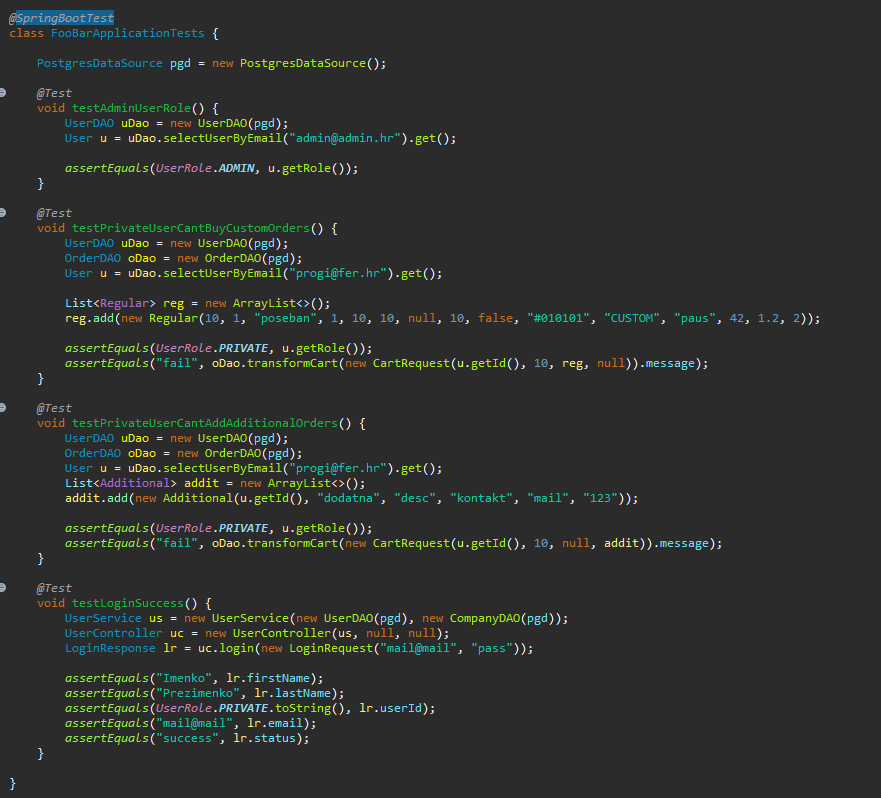
\includegraphics[scale=0.5]{slike/testovi.PNG} 
				\centering
				\caption{Unit testovi}
				\label{fig:unit}%label mora biti drugaciji za svaku sliku
			\end{figure}
			
			\subsection{Ispitivanje sustava}
			
			% \textit{Potrebno je provesti i opisati ispitivanje sustava koristeći radni okvir Selenium\footnote{\url{https://www.seleniumhq.org/}}. Razraditi \textbf{minimalno 4 ispitna slučaja} u kojima će se ispitati redovni slučajevi, rubni uvjeti te poziv funkcionalnosti koja nije implementirana/izaziva pogrešku kako bi se vidjelo na koji način sustav reagira kada nešto nije u potpunosti ostvareno. Ispitni slučaj se treba sastojati od ulaza (npr. korisničko ime i lozinka), očekivanog izlaza ili rezultata, koraka ispitivanja i dobivenog izlaza ili rezultata.\\ }
			 
			 %\textit{Izradu ispitnih slučajeva pomoću radnog okvira Selenium moguće je provesti pomoću jednog od sljedeća dva alata:}
			 %\begin{itemize}
			 	%\item \textit{dodatak za preglednik \textbf{Selenium IDE} - snimanje korisnikovih akcija radi automatskog ponavljanja ispita	}
			 	%\item \textit{\textbf{Selenium WebDriver} - podrška za pisanje ispita u jezicima Java, C\#, PHP koristeći posebno programsko sučelje.}
			 %\end{itemize}
		 	%\textit{Detalji o korištenju alata Selenium bit će prikazani na posebnom predavanju tijekom semestra.}
			
			\eject 
		
		
		\section{Dijagram razmještaja}
			
		%	\textbf{\textit{dio 2. revizije}}
			
			% \textit{Potrebno je umetnuti \textbf{specifikacijski} dijagram razmještaja i opisati ga. Moguće je umjesto specifikacijskog dijagrama razmještaja umetnuti dijagram razmještaja instanci, pod uvjetom da taj dijagram bolje opisuje neki važniji dio sustava.}
			Dijagram razmještaja pruža uvid u topologiju sklopovlja i programsku potporu koja se
			koristi u implementaciji sustava. Klijenti koriste mobilnu aplikaciju kako bi pristupili samoj aplikaciji. Komunikacija između klijenta i poslužitelja bazira se na HTTPS protokolu dok se na poslužiteljskom 
			računalu nalaze web poslužitelj i poslužitelj baze podataka.
			\\
			 \begin{figure}[H]				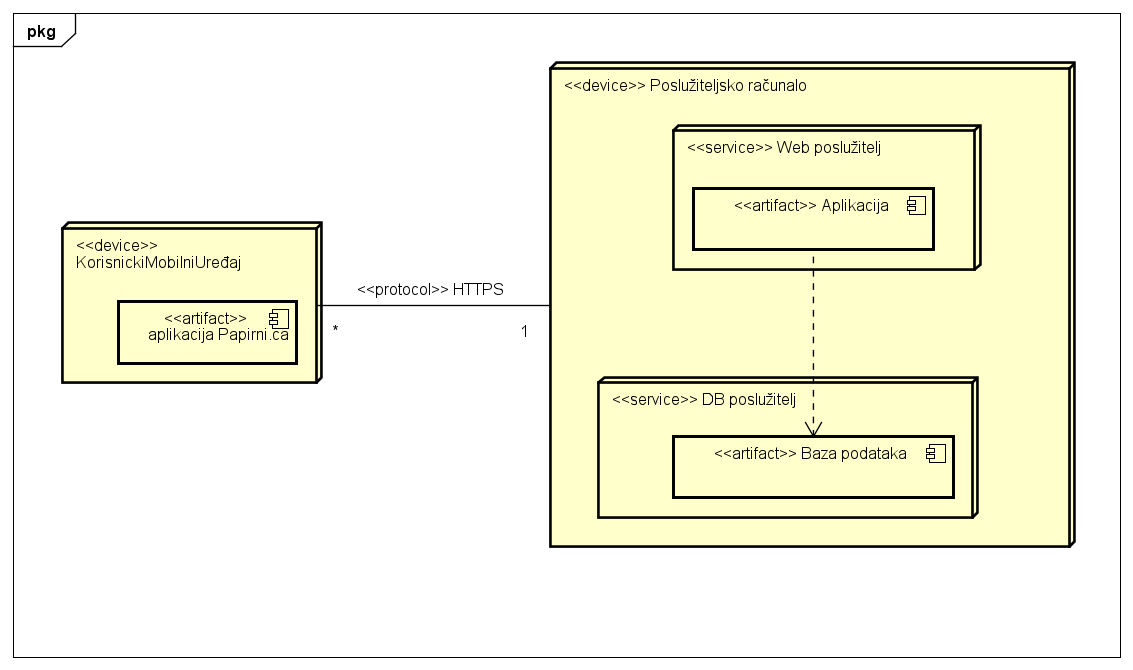
\includegraphics[scale=0.55]{dijagrami/dij_razmjestaj.PNG} 
				\centering
				\caption{Dijagram razmještaja}
				\label{fig:dij_ramjestaj}%label mora biti drugaciji za svaku sliku
			\end{figure}
			
			\eject 
		
		\section{Upute za puštanje u pogon}
			
			\vspace{5mm}
			\noindent \textbf{Izrada Heroku profila}\newline
			Potrebno je napraviti profil na službenim stranicama Herokua.
			
			\vspace{5mm}
			\noindent \textbf{Instalacija Heroku CLI-a}\newline
			Sljedeći korak je sa službene stranice Herokua skinuti Heroku CLI i provesti klasičnu instalaciju.
			
			\vspace{5mm}
			\noindent \textbf{Namještanje i stvaranje Heroku aplikacije}\newline
			Zatim je potrebno otvoriti komandnu liniju i pozicionirati se u direktorij u kojemu će se nalaziti željeni projekt. Pokrenuti naredbu "heroku login" te na upit za otvaranje preglednika kako bi se proveo login stisnuti "q" ako ne 
			želite provesti registraciju, a ako želite stisnite bilo koju preostalu tipku na tipkovnicu. U potvrdnom slučaju se otvara preglednik te je nužno stisnuti "Log In" i prijaviti se. Kako bi se aplikacija stvorila potrebno je u komandnu liniju upisati "git init" pa "heroku create" te se nova aplikacija vašeg profila stvara i ispisuje njeno ime.
			\begin{figure}[H]
				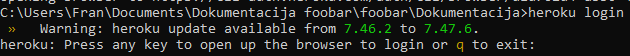
\includegraphics[scale=0.8]{slike/heroku_login.PNG} 
				\centering
				\caption{Upis naredbe za prijavu u Heroku CLI te upit}
				\label{fig:heroku_login}%label mora biti drugaciji za svaku sliku
			\end{figure}
		
			\begin{figure}[H]
				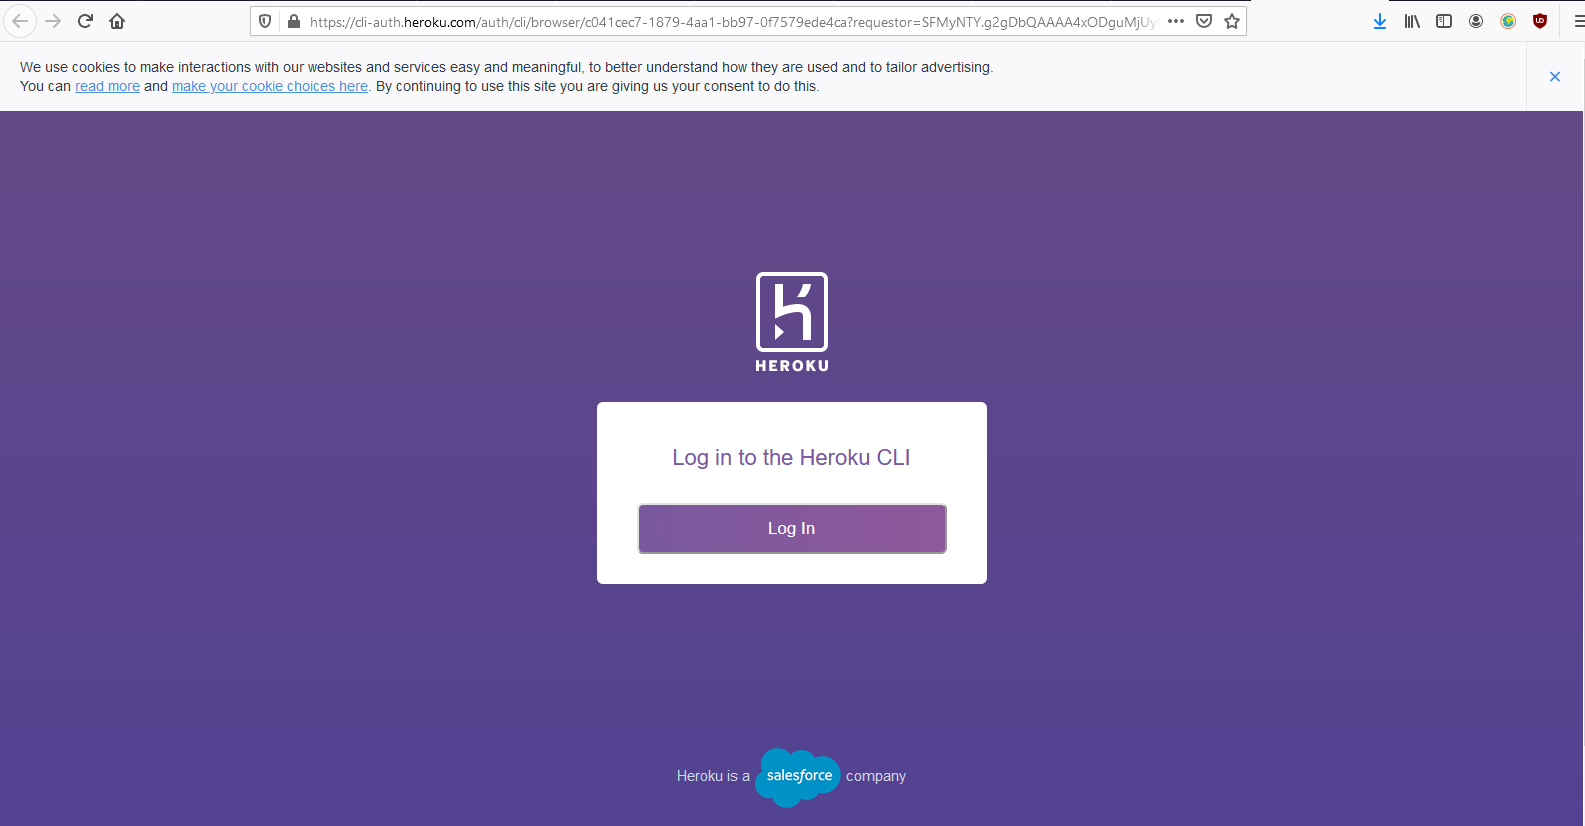
\includegraphics[scale=0.4]{slike/heroku_login_browser.PNG} 
				\centering
				\caption{Otvoreni preglednik za prijavu na Heroku}
				\label{fig:heroku_login_browser}%label mora biti drugaciji za svaku sliku
			\end{figure}
		
			\begin{figure}[H]
				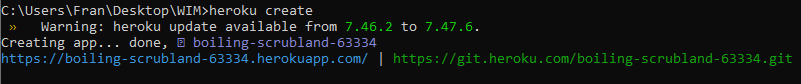
\includegraphics[scale=0.8]{slike/heroku_stvorena_aplikacija.PNG} 
				\centering
				\caption{Naredba za stvaranje nove Heroku aplikacije te ispis dodjeljenog imena}
				\label{fig:heroku_stvorena_aplikacija}%label mora biti drugaciji za svaku sliku
			\end{figure}
			
			\vspace{5mm}
			\noindent \textbf{Namještanje i stvaranje baze podataka na Herokuu}\newline
			Kako bi se stvorila baza podataka u komandnu liniju je potrebno upisati "heroku addons:create heroku-postgresql -a $\langle$APLIKACIJA$\rangle$" gdje je $\langle$APLIKACIJA$\rangle$ ime vaše aplikacije.
			
			\begin{figure}[H]
				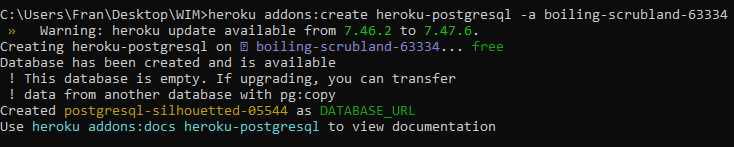
\includegraphics[scale=0.8]{slike/heroku_stvaranje_baze_podataka.PNG} 
				\centering
				\caption{Naredba za stvaranje PostgreSQL baze podataka za Heroku aplikaciju te ispis dodjeljenog imena}
				\label{fig:heroku_stvaranje_baze_podataka}%label mora biti drugaciji za svaku sliku
			\end{figure}
			
			\vspace{5mm}
			 \noindent \textbf{Instalacija PostgreSQL-a}\newline
			 Sa službene stranice je potrebno skinuti i instalirati PostgreSQL i potom staviti PostgreSQL u sistemske varijable.
			 
			 \vspace{5mm}
			 \noindent \textbf{Stvaranje i punjenje baze podataka}\newline
			 Kako bismo imali funkcionalnu bazu podataka potrebno je izmijeniti database\_and\_inserts.sql sa repozitorija tako da promijenimo vrijednosti INSERT naredbe u kojoj se dodaje administrator. Zatim u komandnoj liniji treba pokrenuti "heroku pg:psql -a $\langle$APLIKACIJA$\rangle$" što nas spaja na konzolu baze podataka. Zatim treba jednostavno kopirati i zalijepiti izmijenjeni database\_and\_inserts.sql.
			 
			 \begin{figure}[H]
			 	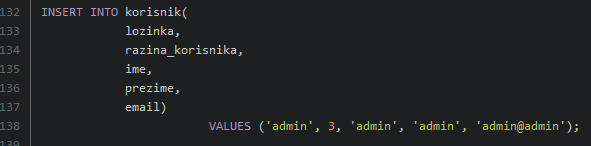
\includegraphics[scale=0.8]{slike/sql_admin.PNG} 
			 	\centering
			 	\caption{Dio SQL upita koji se treba promijeniti u lozinka, 3, ime, prezime i email željenog administratora}
			 	\label{fig:sql_admin}%label mora biti drugaciji za svaku sliku
			 \end{figure}
		 
			 \begin{figure}[H]
			 	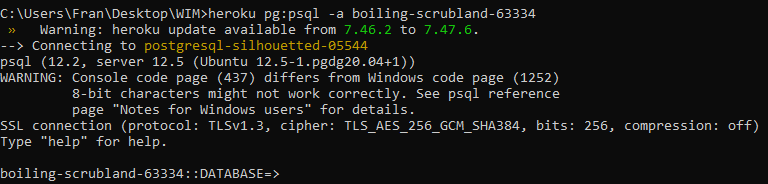
\includegraphics[scale=0.8]{slike/baza_spajanje.PNG} 
			 	\centering
			 	\caption{Naredba za spajanje na stvorenu bazu podataka}
			 	\label{fig:baza_spajanje}%label mora biti drugaciji za svaku sliku
			 \end{figure}
			 
			 \vspace{5mm}
			 \noindent \textbf{Stavljanje backenda na Heroku}\newline
			 Potrebno je skinuti izvorni kod iz direktorija fooBarServer sa repozitorija i staviti ga u direktorij u kojemu smo stvorili Heroku aplikaciju. Zatim treba, pomoću redom "git add .", "git commit -m "$\langle$VASA\_PORUKA$\rangle$"" i  "git push origin master", aplikaciju postaviti na server. To pokreće izgradnju aplikacije te je nakon toga aplikacija spremna za korištenje.
			 
			 \begin{figure}[H]
			 	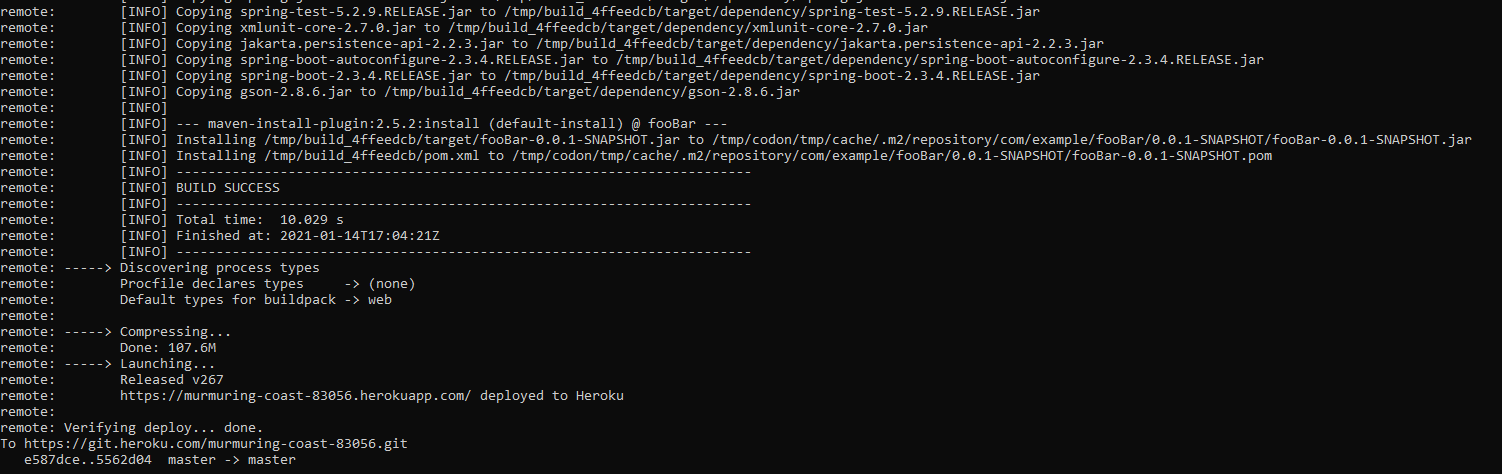
\includegraphics[scale=0.4]{slike/izgradnja_gotova.PNG} 
			 	\centering
			 	\caption{Poruka da se baze uspješno postavila na Heroku}
			 	\label{fig:izgradnja_gotova}%label mora biti drugaciji za svaku sliku
			 \end{figure}
			 
			 \vspace{5mm}
			 \noindent \textbf{Pokretanje mobilne aplikacije} \newline
			 Potrebno je iz direktorija "Izvrsni kod/apk" skinuti aplikacije za mobitel te instalirati onu za Vaš mobilni uređaj. Klikom na ikonu aplikacije Papirni.ca moguće je započeti njeno korištenje.
			 
			\eject 